\begin{example}[二维中 $\mathrm{Re}=20$ 的定常圆柱绕流]\label{ex:appendix-d-5}
该算例由\textcite{SchaeferTurek1996}提出,考虑二维区域中的圆形圆柱绕流,区域示意见图\hyperref[fig:appendix-d-3]{D.3}.
\begin{elegantfigure}[0.75\linewidth]
 \includegraphics[page=760,pagebox=cropbox,trim=79.50bp 248.65bp 79.61bp 351.00bp,clip,width=\linewidth]{../input/source/Finite Element Methods for Incompressible Flow Problems.pdf}
 \captionof{figure}{例题 D.5:计算区域.}\label{fig:appendix-d-3}
\end{elegantfigure}
流体的动力黏度为 $\mu=10^{-3}\,\mathrm{Pa\,s}$,密度为 $\rho=1\,\mathrm{kg/m^3}$,其数值近似对应水.入口采用抛物线速度剖面
\begin{equation}\label{eq:appendix-d-12}
\bm v(0\,\mathrm m,y)
=\frac{1}{0.41^2}
\begin{pmatrix}1.2y(0.41-y)\\0\end{pmatrix}
\frac{\mathrm m}{\mathrm s},
\qquad 0\,\mathrm m\le y\le0.41\,\mathrm m.
\end{equation}
通道上、下壁面以及圆柱表面均施加无滑移条件.出口有两种可选边界条件:抛物线速度
\[
\bm v(2.2\,\mathrm m,y)
=\frac{1}{0.41^2}
\begin{pmatrix}1.2y(0.41-y)\\0\end{pmatrix}
\frac{\mathrm m}{\mathrm s},
\qquad 0\,\mathrm m\le y\le0.41\,\mathrm m,
\]
或 do-nothing 条件
\begin{equation}\label{eq:appendix-d-13}
\bm S\bm n=(\mu\nabla\bm v-P I)\bm n
=\bm 0\,\mathrm{N/m^2}
\qquad\text{于 }\Gamma_{\mathrm{out}},
\end{equation}
其中 $\bm n$ 为指向外侧的单位法向量.入口平均速度为
\[
U_{\mathrm{mean}}
=\frac{1}{0.41^2}
\frac{\int_0^{0.41}1.2y(0.41-y)\,\mathrm dy}
     {\int_0^{0.41}\mathrm dy}\,\frac{\mathrm m}{\mathrm s}
=0.2\,\mathrm{m/s}.
\]
以入口平均速度、圆柱直径 $d=0.1\,\mathrm m$ 及运动黏度 $\mu/\rho$ 为尺度,该流动的 Reynolds 数为 $\mathrm{Re}=20$.外力为零,即 $\bm f^{\mathrm{ext}}=\bm0\,\mathrm{N/m^3}$.此设置存在稳定稳态解,流场见图\hyperref[fig:appendix-d-4]{D.4}和\hyperref[fig:appendix-d-5]{D.5}.
\begin{elegantfigure}[0.84\linewidth]
 \includegraphics[page=761,pagebox=cropbox,trim=52.50bp 112.15bp 52.36bp 437.00bp,clip,width=\linewidth]{../input/source/Finite Element Methods for Incompressible Flow Problems.pdf}
 \captionof{figure}{例题 D.5:圆柱绕流中的速度模(上)和压力(下).}\label{fig:appendix-d-4}
\end{elegantfigure}
\begin{elegantfigure}[0.84\linewidth]
 \includegraphics[page=762,pagebox=cropbox,trim=52.50bp 488.90bp 52.36bp 60.25bp,clip,width=\linewidth]{../input/source/Finite Element Methods for Incompressible Flow Problems.pdf}
 \captionof{figure}{例题 D.5:圆柱表面附近的速度和压力.}\label{fig:appendix-d-5}
\end{elegantfigure}

取特征长度 $L=1\,\mathrm m$、特征速度 $U=1\,\mathrm{m/s}$,可得无量纲稳态 Navier--Stokes 方程\hyperref[eq:steady-ns-strong]{(6.1)}中的黏度 $\nu=\mu/(\rho UL)=10^{-3}$,入口条件
\[
\bm u(0,y)=\frac{1}{0.41^2}
\begin{pmatrix}1.2y(0.41-y)\\0\end{pmatrix},
\qquad 0\le y\le0.41,
\]
以及出口条件
\begin{equation}\label{eq:appendix-d-14}
\bm u(2.2,y)=\frac{1}{0.41^2}
\begin{pmatrix}1.2y(0.41-y)\\0\end{pmatrix},
\qquad 0\le y\le0.41,
\end{equation}
或
\begin{equation}\label{eq:appendix-d-15}
(\nu\nabla\bm u-pI)\bm n=\bm0
\qquad\text{于 }\Gamma_{\mathrm{out}}.
\end{equation}

感兴趣的量是物体所受的力,具体而言是阻力系数\hyperref[eq:appendix-d-3]{(D.3)}和升力系数\hyperref[eq:appendix-d-6]{(D.6)}.本二维算例中,主流方向为 $\bm w_{\mathrm{drag}}=(1,0)^\mathsf T$,与之正交的方向为 $\bm w_{\mathrm{lift}}=(0,1)^\mathsf T$;相对速度取 $V=U_{\mathrm{mean}}$,参考面积取圆柱直径 $A=d$.

笔记\hyperref[note:appendix-d-2]{D.2}介绍了计算阻力和升力系数的两种方法.由于圆柱是圆形,有限元网格无法精确表示其边界,若使用边界积分公式\hyperref[eq:appendix-d-4]{(D.4)}和\hyperref[eq:appendix-d-7]{(D.7)},仅边界近似就可能带来显著误差.因此应优先使用面积积分公式\hyperref[eq:appendix-d-5]{(D.5)}和\hyperref[eq:appendix-d-8]{(D.8)}.该算例为稳态问题且 $\bm f=0$,故对任意满足
$\bm w_{\mathrm{drag}}\in H^1(\Omega)^2$、在 $\partial\Omega\setminus\Gamma_{\mathrm{body}}$ 上为零且在 $\Gamma_{\mathrm{body}}$ 上取值 $(1,0)^\mathsf T$ 的函数,有
\begin{equation}\label{eq:appendix-d-16}
c_{\mathrm{drag}}
=-500\left[
(\nu\nabla\bm u,\nabla\bm w_{\mathrm{drag}})
+n(\bm u,\bm u,\bm w_{\mathrm{drag}})
-(\nabla\cdot\bm w_{\mathrm{drag}},p)
\right].
\end{equation}
这里采用稳态模拟中常见的黏性项形式,而 $n(\bm u,\bm u,\bm w_{\mathrm{drag}})$ 可取第\hyperref[subsec:steady-ns-nonlinear-term]{6.1.2}节介绍的任一种对流项形式.类似地,对任意在 $\partial\Omega\setminus\Gamma_{\mathrm{body}}$ 上为零、且在 $\Gamma_{\mathrm{body}}$ 上等于 $(0,1)^\mathsf T$ 的 $\bm w_{\mathrm{lift}}\in H^1(\Omega)^2$,有
\begin{equation}\label{eq:appendix-d-17}
c_{\mathrm{lift}}
=-500\left[
(\nu\nabla\bm u,\nabla\bm w_{\mathrm{lift}})
+n(\bm u,\bm u,\bm w_{\mathrm{lift}})
-(\nabla\cdot\bm w_{\mathrm{lift}},p)
\right].
\end{equation}

另一个感兴趣的量是圆柱前后两点间的压力差
\[
\Delta P=P(0.15,0.2)-P(0.25,0.2),
\]
其无量纲形式为
\begin{equation}\label{eq:appendix-d-18}
\Delta P=\rho U^2\bigl(p(0.15,0.2)-p(0.25,0.2)\bigr).
\end{equation}
当出口采用 Dirichlet 条件\hyperref[eq:appendix-d-14]{(D.14)}时,\textcite{JohnMatthies2001} 给出了相当准确的参考值:
\begin{equation}\label{eq:appendix-d-19}
c_{\mathrm{drag,ref}}=5.57953523384.
\end{equation}
\begin{equation}\label{eq:appendix-d-20}
c_{\mathrm{lift,ref}}=0.010618937712.
\end{equation}
\begin{equation}\label{eq:appendix-d-21}
\Delta p_{\mathrm{ref}}=0.11752016697.
\end{equation}
若出口采用 do-nothing 条件\hyperref[eq:appendix-d-15]{(D.15)},阻力系数和压力差参考值不变,升力系数则对出口条件稍敏感.\textcite{Nabh1998} 给出的升力系数参考值为
\begin{equation}\label{eq:appendix-d-22}
c_{\mathrm{lift,ref}}=0.010618948146.
\end{equation}
\end{example}

\begin{example}[三维中 $\mathrm{Re}=20$ 的定常圆柱绕流]\label{ex:appendix-d-6}
该问题是例题\hyperref[ex:appendix-d-5]{D.5} 的三维扩展,也由\textcite{SchaeferTurek1996}提出.区域为图\hyperref[fig:appendix-d-6]{D.6}所示、带圆柱的通道.通道高度为 $H=0.41\,\mathrm m$,圆柱直径为 $d=0.1\,\mathrm m$.没有外力,动量方程右端为 $\bm f=0$.流体的动力黏度为 $\mu=10^{-3}\,\mathrm{Pa\,s}$,密度为 $\rho=1\,\mathrm{kg/m^3}$.入口条件为
\[
\bm v|_{\mathrm{in}}
=\frac{1}{H^4}
\begin{pmatrix}
16Uyz(H-y)(H-z)\\0\\0
\end{pmatrix}\mathrm{m/s},
\qquad U=0.45\,\mathrm{m/s}.
\]
入口平均速度为
\[
U_{\mathrm{mean}}
=\frac{\int_0^H\int_0^H v_{\mathrm{in},1}\,\mathrm dy\,\mathrm dz}
        {\int_0^H\int_0^H\mathrm dy\,\mathrm dz}
=\frac{16\cdot0.45}{36}=0.2\,\mathrm{m/s}.
\]
因此,以 $U_{\mathrm{mean}}$、圆柱直径 $d$ 及运动黏度 $\mu/\rho$ 为尺度,该流动的 Reynolds 数为 $\mathrm{Re}=20$.
\begin{elegantfigure}[0.92\linewidth]
 \includegraphics[page=764,pagebox=cropbox,trim=79.00bp 394.15bp 79.86bp 60.25bp,clip,width=\linewidth]{../input/source/Finite Element Methods for Incompressible Flow Problems.pdf}
 \captionof{figure}{例题 D.6:三维圆柱绕流计算区域.}\label{fig:appendix-d-6}
\end{elegantfigure}
取 $L=1\,\mathrm m$ 和 $U=1\,\mathrm{m/s}$,得到无量纲稳态 Navier--Stokes 方程\hyperref[eq:steady-ns-strong]{(6.1)},其中 $\nu=\mu/(\rho UL)=10^{-3}$.出口可采用与入口相同的速度条件,也可采用某种 do-nothing 条件;其余边界均施加无滑移条件 $\bm u=0$.与二维情形(例题\hyperref[ex:appendix-d-5]{D.5})一样,圆柱后方形成反向旋转的涡旋.若考察剖面,例如 $z=0.41/2$,流场形态与图\hyperref[fig:appendix-d-4]{D.4}和\hyperref[fig:appendix-d-5]{D.5}类似.

感兴趣的量为圆柱受到的阻力系数、升力系数及压力差
\begin{equation}\label{eq:appendix-d-23}
\Delta p=p(0.45,0.2,0.205)-p(0.55,0.2,0.205).
\end{equation}
阻力和升力系数的计算见笔记\hyperref[note:appendix-d-2]{D.2}.有限元方法需近似圆柱边界,因此应优先使用体积分.不过,此处物体与区域其余边界相连,故 $\bm w_{\mathrm{drag}}$ 和 $\bm w_{\mathrm{lift}}$ 的定义必须作折衷.例如,\textcite{John2002} 将 $\bm w_{\mathrm{drag}}$ 定义为与速度有限元多项式次数相同的有限元函数.圆柱边界上所有自由度——包括圆柱与区域左右边界交接处的自由度——都赋值为 $(1,0,0)^\mathsf T$;其余自由度赋值为零.$\bm w_{\mathrm{lift}}$ 采用相同构造,只是圆柱边界自由度取 $(0,1,0)^\mathsf T$.随后在\hyperref[eq:appendix-d-5]{(D.5)}和\hyperref[eq:appendix-d-8]{(D.8)}中取 $A=dH=0.041\,\mathrm{m^2}$、$V=U_{\mathrm{mean}}$,得到
\[
\begin{aligned}
c_{\mathrm{drag}}
&=-\frac{500}{0.41}\left[
(\nu\nabla\bm u,\nabla\bm w_{\mathrm{drag}})
+n(\bm u,\bm u,\bm w_{\mathrm{drag}})
-(\nabla\cdot\bm w_{\mathrm{drag}},p)\right],\\
c_{\mathrm{lift}}
&=-\frac{500}{0.41}\left[
(\nu\nabla\bm u,\nabla\bm w_{\mathrm{lift}})
+n(\bm u,\bm u,\bm w_{\mathrm{lift}})
-(\nabla\cdot\bm w_{\mathrm{lift}},p)\right].
\end{aligned}
\]
使用 Gaussian 等求积公式在单元内部计算系数时,$\bm w_{\mathrm{drag}}$ 和 $\bm w_{\mathrm{lift}}$ 的修改不会直接进入数值积分(求积点不会落在网格单元边界上),因此这种修改影响甚微.表\hyperref[tab:appendix-d-1]{D.1}列出了\textcite{SchaeferTurek1996} 给出的参考区间和\textcite{John2002} 给出的参考值.
\begin{eleganttable}
\captionof{table}{例题 D.6 的阻力系数、升力系数和压力差参考值.}\label{tab:appendix-d-1}
\begin{tabular}{lcc}
\toprule
量 & Schäfer 和 Turek(1996) & John(2002)\\
\midrule
$c_{\mathrm{drag}}$ & $[6.05,6.25]$ & $6.1853329$\\
$c_{\mathrm{lift}}$ & $[0.008,0.01]$ & $0.0094009839$\\
$\Delta p$ & $[0.165,0.175]$ & $0.1708$\\
\bottomrule
\end{tabular}
\end{eleganttable}
\end{example}
